\subsection{Publizierung}
Um mit dem Produkt etwas zu erwirtschaften, muss dieses der Zielgruppe anschaulich gemacht werden. Dabei ist die größe der Plattformen und die Anzahl der Plattformen, welche dies machen, für ein erfolgreiches Produkt besonders wichtig.
\paragraph{Aktivitätsdiagramm Publizierung}\mbox{}\\
\begin{figure}[H]
	\centering
	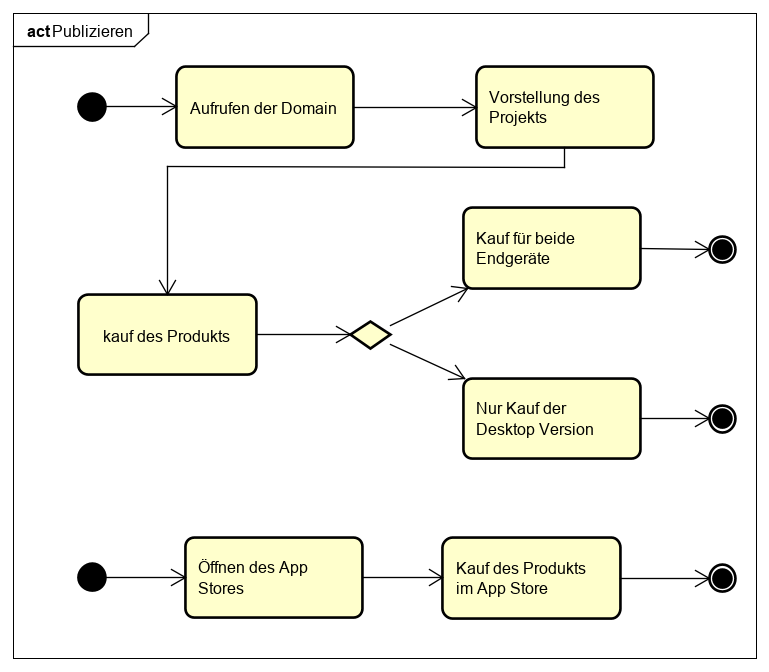
\includegraphics[width= 0.9\linewidth]{diagramms/activity/Publizieren.png}
	\caption{Aktivitätsdiagramm Publizierung}
\end{figure}
\newpage
\begin{indentE}\mbox{}
	\paragraph{/LF3110/ Website erstellen}\mbox{}\\
	Es wird eine Webseite erstellt, auf welche das Produkt vorgestellt wird. Außerdem soll diese dem Besucher das Projektteam und den Auftraggeber näher bringen, auf einer eigenen About-Seite. Diese Webseite wird dann auf einen Hosting-Provider hochgeladen, von wo sie mit einer Domain aufgerufen werden kann.
	\UseCase{
		{Publizierung}
		{/LF3110/ Website erstellen}
		{Publizierung}
		{Es wird eine Webseite erstellt, auf welche das Produkt publiziert werden soll. Diese soll außerdem auf das Projektteam aufmerksam machen und über das Internet mit einer Domain erreichbar sein.}
		{Das Produkt soll auf einer Webseite publiziert werden, und den potenziellen Kunden das Projektteam näher gebracht werden.}
		{Das Produkt ist im Internet auffindbar}
		{Benutzer, Projektteam (Auftraggeber + Auftragnehmer)}
		{Produktinformationen, Projektteam}
		{Das Produkt kann nicht über eine Webseite aufgefunden werden.}
		{Das Produkt ist über ein Webseite auffindbar}
		{hoch}
		{gering}
		{Must Have}
	}
	\paragraph{/LF3120/ Produkt auf Webseite veröffentlichen}\mbox{}\\
	Das Produkt muss auf ihrer eigenen Webseite /LF2060/ publiziert werden. Diese besitzt eine eigne Seite für den Download der Software. Dort kann man die App und Desktop Version für 5€ kaufen und die Desktop Version einzeln für 3€.
	\UseCase{
		{Publizierung}
		{LF3120/ Produkt auf Webseite veröffentlichen}
		{Publizierung}
		{Das Produkt soll von der Webseite gedownloadet werden können. Dabei soll die App und Desktop Version für 5 € gemeinsame und die Desktop Version einzeln für 3€ angeboten werden.}
		{Das Produkt muss für den potenziellen Kunden erwerbbar sein}
		{Das Produkt kann auf der Webseite automatisiert verkauft werden}
		{potenzieller Kunde}
		{Zahlungsinformationen, Produkt (als Download)}
		{Das Produkt ist für den potenziellen Kunden nicht erwerbbar}
		{Das Produkt kann auf der Webseite verwirtschaftet werden}
		{hoch}
		{mittel}
		{Must Have}
	}
	\paragraph{/LF3210/ Produkt auf Play Store veröffentlichen}\mbox{}\\
	Die Android App soll auf dem Google Play Store hochgeladen werden und dort für eine Preis von 3€ verkauft werden. Dafür muss ein Google Developer Account erstellt werden, um diese hochzuladen.
	\UseCase{
		{Publizierung}
		{/LF3210/ Produkt auf Play Store veröffentlichen}
		{Publizierung}
		{Die App-Version wird auf dem Play Store veröffentlicht, wo sie für 3€ erwerbt werden kann.}
		{Es soll die potenzielle Kundschaft erhöht werden, indem ie App-Version auch auf dem Play-Store verfügbar ist.}
		{Es wird eine größter Kundschaft(Android) angesprochen}
		{potenzielle Kunden}
		{App-Version(als Download)}
		{Der Erwerb wird nicht auf dem Play Store angeboten.}
		{Der Erwerb ist über den Play Store möglich}
		{mittel}
		{gering}
		{Should Have}
	}
	\paragraph{/LF3220/ Produkt auf App Store veröffentlichen}\mbox{}\\
	Die iOS App kann auf dem Apple App Store hochgeladen werden und dort für 3€ verkauft werden.
	\UseCase{
		{Publizierung}
		{/LF3220/ Produkt auf App Store veröffentlichen}
		{Publizierung}
		{Die App-Version wird auf dem App Store veröffentlicht, wo sie für 3€ erwerbt werden kann.}
		{Es soll die potenzielle Kundschaft erhöht werden, indem ie App-Version auch auf dem App Store verfügbar ist.}
		{Es wird eine größter Kundschaft(iOS) angesprochen}
		{potenzielle Kunden}
		{App-Version(als Download)}
		{Der Erwerb wird nicht auf dem App Store angeboten.}
		{Der Erwerb ist über den App Store möglich}
		{mittel}
		{mittel}
		{Nice to Have}
	}
\end{indentE}